\begin{parts}
	\part

	Describa cuatro términos de la serie de Taylor de una función real
	de variable real infinitamente diferenciable en un dominio
	adecuado.

	\part

	Describa cuatro términos de la serie de una función real de dos
	variables reales infinitamente diferenciable en un dominio
	adecuado.

	\part

	Describa el gradiente y el hessiano de una función real de tres
	variables reales en un dominio adecuado.
\end{parts}

\begin{figure}[ht!]
	\centering
	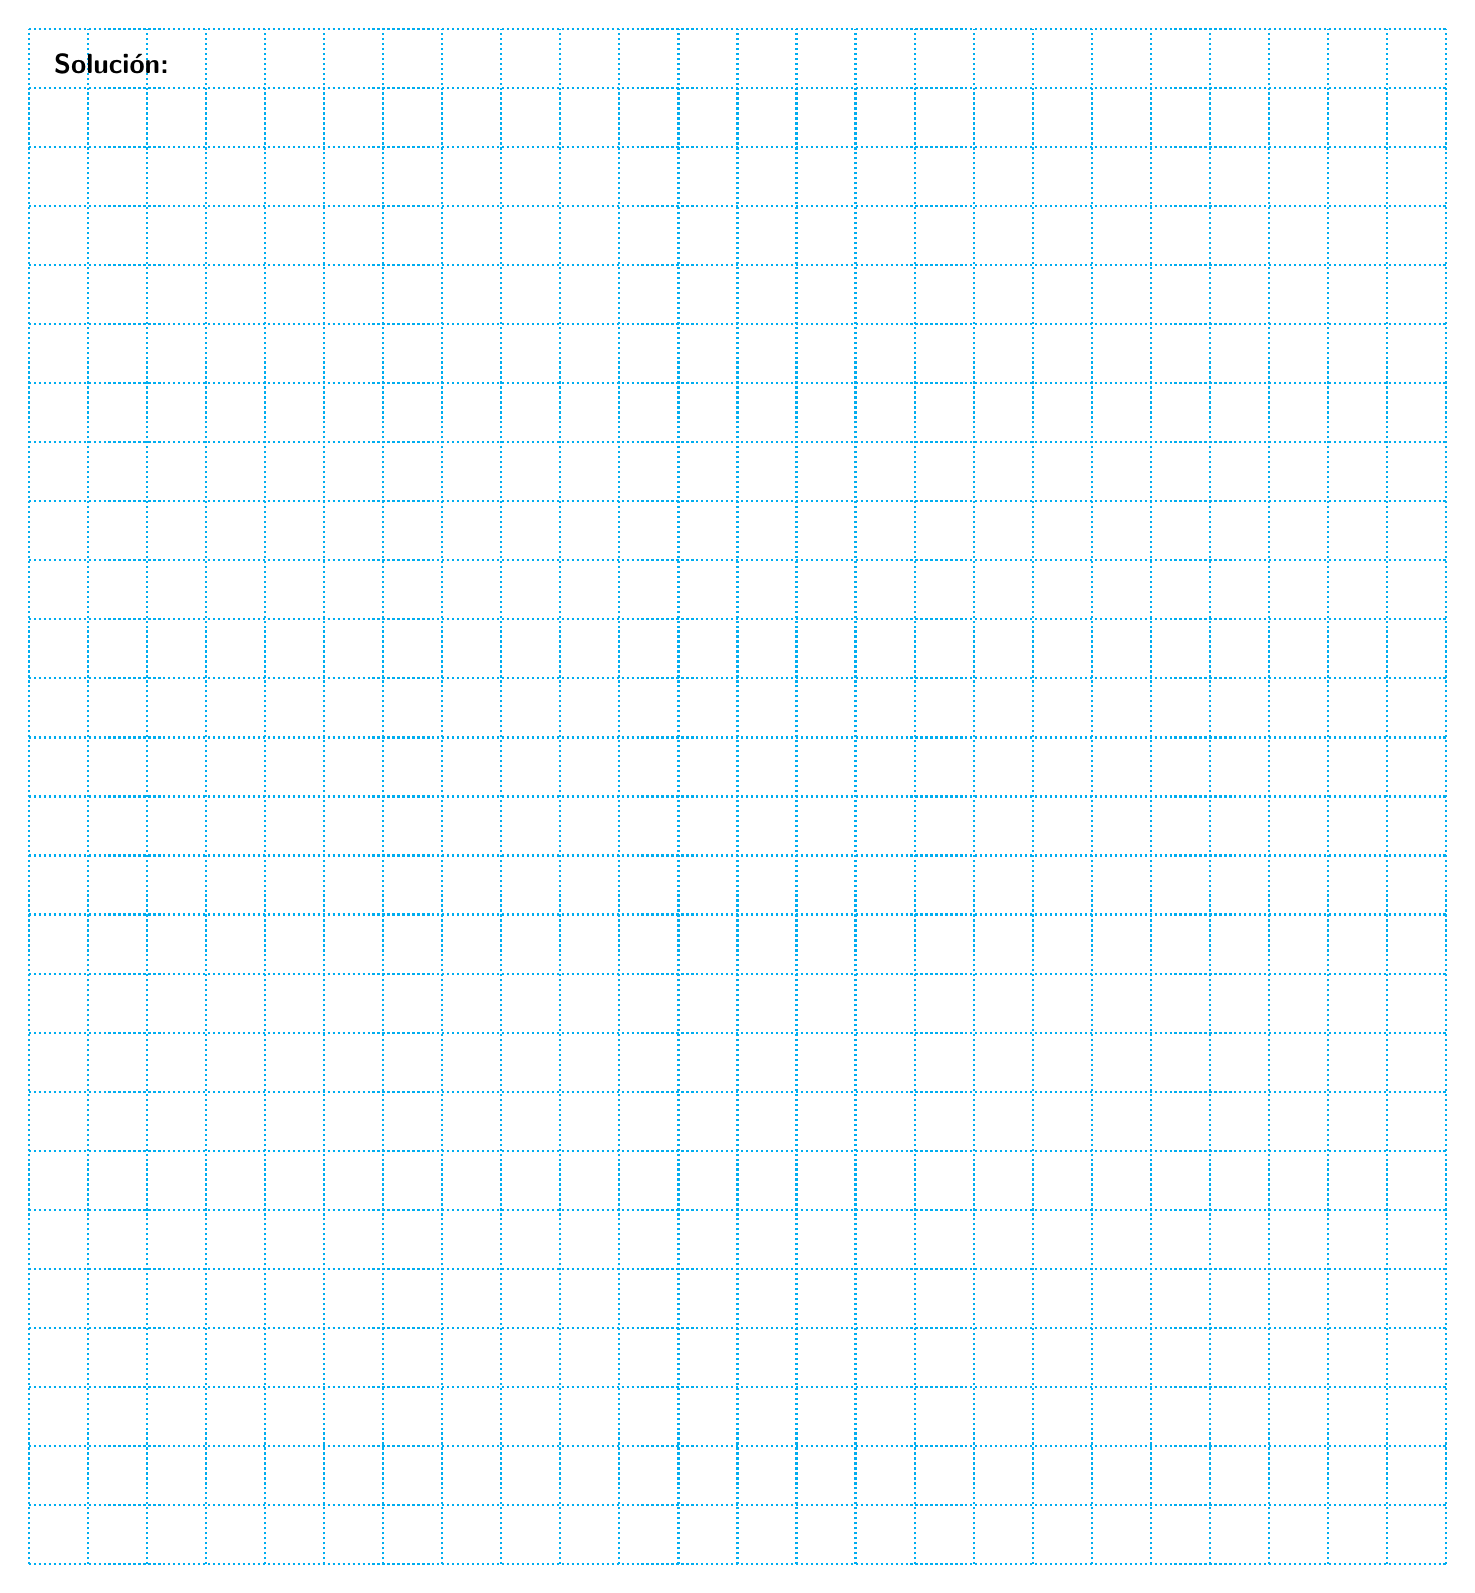
\begin{tikzpicture}[xscale=0.75,yscale=0.75]
		\draw[help lines,color=cyan,thick,densely dotted] (0,0) grid (24,26);
		\draw (1.4,25.4) node {\textsf{\bfseries Solución:}};
	\end{tikzpicture}
\end{figure}

